\section{Training Procedure of DeltaKV}
\label{app:training}

Algorithm \ref{alg:DeltaKV} details the training workflow of the DeltaKV framework, which optimizes the compression and decompression modules alongside the frozen LLM backbone. The procedure consists of three steps:

\begin{itemize}[nolistsep, left=0pt]
  \item \textbf{Ground Truth Forward:} 
  The model first performs a standard forward pass using the original uncompressed KV cache to generate the target KV representations and logits.
  
  \item \textbf{DeltaKV Forward \& Reconstruction:} 
  In this step, the algorithm iterates through each layer and token sequence. For every current token, it retrieves the top-$k$ most similar historical tokens from a strided reference set $\mathcal{T}_{ref}$ based on the $L_2$ distance. The mean of these references, $\overline{KV}_R$, is subtracted from the current token's representation to form a residual. This residual is compressed into a low-dimensional latent vector $z_{\Delta}$ via the compressor $f_c$ and subsequently reconstructed by the decompressor $f_d$. The final approximated KV state, $\hat{kv}_i$, is obtained by adding the reconstructed residual back to the mean reference.
  
  \item \textbf{End-to-End Loss Calculation:} 
  The training objective combines two loss functions: a reconstruction loss ($\mathcal{L}_{rec}$), which minimizes the Mean Squared Error (MSE) between the original and reconstructed KV states, and a Next Token Prediction loss ($\mathcal{L}_{ntp}$), which ensures the compressed cache maintains the model's generative capabilities. The total loss is computed as $\mathcal{L} = \mathcal{L}_{rec} + \mathcal{L}_{ntp}$.
\end{itemize}

\begin{algorithm}[ht]
% \small
\caption{Training Procedure of DeltaKV}
\label{alg:DeltaKV}
\KwIn{
Input token sequence $\mathcal{T}$; number of layers $L$; frozen LLM parameters $\Theta$; trainable compressor $f_\mathrm{c}$; trainable decompressor $f_\mathrm{d}$; stride $s$; number of references $k$;
}
\KwOut{Total loss $\mathcal{L}$;}
\step{Step 1: Ground Truth Forward}
$\{\bm{KV}, \cdots\} \gets \mathrm{Forward}(\mathcal{T}, \Theta)$ \cmt{Cache original KV states}

\step{Step 2: DeltaKV Forward \& Reconstruction}
$\mathcal{L}_{\mathrm{rec}} \gets 0$; $\bm{h} \gets \mathrm{Embed}(\mathcal{T})$\;

\For{$l=1$ \KwTo $L$}{
    $\mathcal{T}_{\mathrm{ref}} \gets \emptyset$\;

    $\bm{KV}^{\mathrm{cur}} \gets \mathrm{Proj}(\bm{h}, \Theta_l)$ \cmt{Compute current-layer KV for all tokens}

    \For{$i=1$ \KwTo $|\mathcal{T}|$}{
        $\bm{kv}_i \gets \bm{KV}^{\mathrm{cur}}[i]$

        $\mathcal{R}_i \gets \mathop{\mathrm{arg~top}k}_{\bm{kv}_{\mathrm{ref}} \in \mathcal{T}_{\mathrm{ref}}} \left( - \|\bm{kv}_i - \bm{kv}_{\mathrm{ref}}\|_2^2 \right)$\;
        $\overline{\bm{KV}}_{R} \gets \mathrm{Mean}(\mathcal{R}_i)$ \cmt{Mean of retrieved references}

        $\bm{z}_\Delta \gets f_\mathrm{c}(\bm{kv}_i) - f_\mathrm{c}(\overline{\bm{KV}}_{R})$ \cmt{Latent residual}
        
        $\widehat{\bm{KV}}_\Delta \gets f_\mathrm{d}(\bm{z}_\Delta)$\;
        $\widehat{\bm{kv}}_i \gets \widehat{\bm{KV}}_\Delta + \overline{\bm{KV}}_{R}$ \cmt{Reconstruct KV}
        $\widehat{\bm{KV}}^{\mathrm{cur}}[i] \gets \widehat{\bm{kv}}_i$\;

        $\mathcal{L}_{\mathrm{rec}} \gets \mathcal{L}_{\mathrm{rec}} + \|\bm{KV}_l[i] - \widehat{\bm{kv}}_i\|^2$\;

        \If{$i \bmod s = 0$}{
            $\mathcal{T}_{\mathrm{ref}} \gets \mathcal{T}_{\mathrm{ref}} \cup \{\widehat{\bm{kv}}_i\}$ \cmt{Reference set: only tokens with index $i \bmod s = 0$}
        }
    }
    $\bm{h} \gets \mathrm{AttnFFN}(\bm{h}, \widehat{\bm{KV}}^{\mathrm{cur}}, \Theta_l)$\; 
}
 \step{Step 3: End-to-End Loss Calculation}
$\bm{O}^{\mathrm{DeltaKV}} \gets \mathrm{LMHead}(\bm{h})$\;
$\mathcal{L}_{\mathrm{ntp}} \gets \mathrm{CrossEntropy}(\bm{O}^{\mathrm{DeltaKV}}, \mathcal{T}_{\mathrm{next}})$\;
$\mathcal{L} \gets \mathcal{L}_{\mathrm{rec}} + \mathcal{L}_{\mathrm{ntp}}$ \cmt{Joint optimization}
\Return $\mathcal{L}$\;
\end{algorithm}
\setlength{\textfloatsep}{1.0em}


% =========================
% Algo (one-column friendly)
% =========================

% \begin{algorithm}[t]
% % \small
% \caption{Training Procedure of DeltaKV}
% \label{alg:DeltaKV}
% \KwIn{
% Input token sequence $\mathcal{T}$; number of layers $L$; frozen LLM parameters $\Theta$; trainable compressor $\phi_c$; trainable decompressor $\phi_d$; stride $s$; number of references $k$; weight $\lambda$\;
% }
% \KwOut{Total loss $\mathcal{L}$;}
% % \step{Step 1: Ground Truth Forward (Teacher)}
% $\{\bm{KV}^{\mathrm{GT}}, \cdots\} \gets \mathrm{Forward}(\mathcal{T}, \Theta)$\; 

% % \step{Step 2: DeltaKV Forward \& Reconstruction (Student)}
% $\mathcal{L}_{\mathrm{rec}} \gets 0$; $\bm{h} \gets \mathrm{Embed}(\mathcal{T})$\;

% \For{$l=1$ \KwTo $L$}{
%     $\mathcal{T}_{\mathrm{ref}} \gets \emptyset$

%     $\bm{KV}^{\mathrm{cur}} \gets \mathrm{Proj}(\bm{h}, \Theta_l)$\; % 

%     \For{$i=1$ \KwTo $|\mathcal{T}|$}{
%         $\mathcal{R}_i \gets \mathrm{TopkSimilar}(\bm{KV}^{\mathrm{cur}}[i], \mathcal{T}_{\mathrm{ref}}, k)$\;
%         $\overline{\bm{KV}}_{R} \gets \mathrm{Mean}(\mathcal{R}_i)$\; % 

%         $\bm{P} \gets \phi_c(\bm{KV}^{\mathrm{cur}}[i]) - \phi_c(\overline{\bm{KV}}_{R})$\; % 
%         $\widehat{\bm{KV}}^{\mathrm{cur}}[i] \gets \phi_d(\bm{P}) + \overline{\bm{KV}}_{R}$\; % 

%         $\mathcal{L}_{\mathrm{rec}}\!\gets\!\mathcal{L}_{\mathrm{rec}}\!+\!\mathrm{MSE}(\widehat{\bm{KV}}^{\mathrm{cur}}[i], \bm{KV}^{\mathrm{GT}}_l[i])$\;

%         \If{$i \bmod s = 0$}{
%             $\mathcal{T}_{\mathrm{ref}} \gets \mathcal{T}_{\mathrm{ref}} \cup \{\widehat{\bm{KV}}^{\mathrm{cur}}[i]\}$\;
%         }
%     }
%     $\bm{h} \gets \mathrm{AttnFFN}(\bm{h}, \widehat{\bm{KV}}^{\mathrm{cur}}, \Theta_l)$\; 
% }
% %  \step{Step 3: End-to-End Loss Calculation}
% $\bm{O}^{\mathrm{DeltaKV}} \gets \mathrm{LMHead}(\bm{h})$\;
% $\mathcal{L}_{\mathrm{ntp}} \gets \mathrm{CrossEntropy}(\bm{O}^{\mathrm{DeltaKV}}, \mathcal{T}_{\mathrm{next}})$\;
% $\mathcal{L} \gets \mathcal{L}_{\mathrm{rec}} + \lambda \mathcal{L}_{\mathrm{ntp}}$\; 

% \Return $\mathcal{L}$\;
% \end{algorithm}






\section{Implementation Details of Sparse-vLLM}
\label{app:sparse_vllm}

This appendix provides the technical specifications of the Sparse-vLLM architecture, focusing on the data structures and algorithmic workflows that enable the modularity described in the main text.


\subsection{CacheManager Data Structures}
\label{app:sparse_vllm:structures}

The \texttt{CacheManager} features an extensible architecture where internal data layouts can be customized to match the memory access patterns of emerging algorithms. To demonstrate this flexibility, we currently provide implementations for three representative storage backends catering to physical eviction, logical masking, and hybrid compression paradigms:

\paragraph{Per-Layer Independent Mapping (for Physical Eviction)} 
Algorithms like SnapKV and PyramidKV diverge in their token retention across layers. To support this without approximation errors, the \texttt{CacheManager} instantiates $L$ independent page tables (where $L$ is the number of layers). Each table is a tensor \texttt{buffer\_req\_to\_token\_slots[layer\_idx]}, mapping logical positions to physical slots. While this increases metadata memory usage by a factor of $L$, it is strictly necessary for algorithms where the "KV view" is physically discontinuous and unique per layer.

\paragraph{Global Shared Mapping (for Logical Masking)} 
For Full Attention and OmniKV, where tokens are retained globally but masked logically, we maintain a unified \texttt{req\_to\_token\_slots} table shared across all layers. This minimizes metadata overhead and maximizes cache locality for the mapping tables during kernel execution.

\paragraph{Heterogeneous DeltaKV Storage} 
For DeltaKV, the \texttt{CacheManager} introduces a tiered storage system to handle the duality of raw and compressed data:
\begin{itemize}[nolistsep, left=0pt]
  \item \textbf{Dual Physical Pools}: It manages a \texttt{Full Pool} for high-precision tokens (Sink/Recent) and a separate \texttt{Latent Pool} for compressed vectors. The system dynamically allocates slots from these pools based on the token's lifecycle state.
  
  \item \textbf{Intra-Group Slot Sharing}: To optimize the Observation-Sparse layer groups, the manager implements a ``Copy-on-Write'' style mechanism for reconstruction. When an Observation Layer identifies Top-K tokens, the subsequent sparse layers share the underlying temporary slots allocated for reconstruction. This prevents redundant decompression operations within the same group, significantly reducing the memory bandwidth pressure during the pre-forward phase.
\end{itemize}



\subsection{Sparse Controller Workflows}
\label{app:sparse_vllm:workflows}

The Sparse Controller orchestrates the interaction between the model and the CacheManager. 
Below, we detail the specific workflow implemented for the DeltaKV mechanism:

\paragraph{DeltaKV View Construction (Pre-Forward)}
Unlike standard retrieval, DeltaKV requires on-the-fly reconstruction. The Controller executes the following pipeline before the attention operation:
\begin{enumerate}[nolistsep,label*=(\arabic*)]
  \item \textbf{Index Resolution}: Based on the reference tokens, the Controller identifies the logical indices of tokens requiring decompression.
  
  \item \textbf{Batch Reconstruction}: It instructs the \texttt{CacheManager} to fetch compressed vectors from the \texttt{Latent Pool} and their corresponding references.
  
  \item \textbf{Slot Virtualization}: The reconstructed KV pairs are written to a temporary physical buffer. The Controller then constructs a virtual \texttt{slot\_mapping} that stitches together the static slots (Sink/Recent) and these temporary dynamic slots, presenting a contiguous logical view to the attention kernel.
\end{enumerate}

\paragraph{DeltaKV Lifecycle Management (Post-Forward)}
To handle the transition from high-precision to compressed storage, the Controller monitors the \texttt{Recent Buffer} boundary. Upon buffer overflow, it triggers a specialized fused kernel that:
\begin{enumerate}[nolistsep,label*=(\arabic*)]
  \item Computes the residual between the overflowed token and its assigned reference tokens.
  
  \item Compresses the residual via the down-projection encoder.
  
  \item Writes the result to the \texttt{Latent Pool} and frees the original \texttt{Full Pool} slots immediately, ensuring constant memory complexity relative to sequence length.
\end{enumerate}



\subsection{Kernel Optimizations}
\label{app:sparse_vllm:optimizations}

While we leverage standard high-performance operators (e.g., FlashAttention with indirect addressing), DeltaKV necessitates specific kernel optimizations to minimize overhead:

\begin{itemize}[nolistsep, left=0pt]
  \item \textbf{Indirect Addressing via Slot Mapping}: We modified the Flash-Decoding kernels to accept a token-level \texttt{req\_to\_token\_slots} index array. This allows the attention mechanism to read directly from non-contiguous physical memory locations without intermediate copy operations or block-table lookups.
  
  \item \textbf{Fused DeltaKV Kernels}: We implemented custom Triton kernels to accelerate the compression/decompression loop. This includes a \textbf{Batch L2 Distance} kernel for rapid reference searching and a \textbf{Fused Reconstruction} kernel that combines the gathering of reference tokens, mean calculation, and residual addition into a single kernel launch to minimize GPU memory bandwidth consumption. In the main text, except for the configurations used in ablation studies, the reference stride is generally set to $s=10$. This implies that even for a sequence of 1M tokens, there are only approximately 100k references, and performing efficient matrix multiplication on the GPU remains remarkably fast. Consequently, we did not consider employing approximate algorithms such as Approximate Nearest Neighbors (ANN).
\end{itemize}


\subsection{Potential Memory Efficiency}
\label{app:sect:mem_eff}

Although DeltaKV already achieves significant memory reduction ($\approx 29\%$), there remains substantial headroom for further optimization. Currently, to guarantee near-lossless performance and simplify engineering implementation, we strictly limit quantization to the compressed residuals $z_{\Delta}$, while keeping both the reference tokens and the full attention layers in high precision (e.g., BF16). 

\paragraph{Full-Pipeline Quantization.}
Integrating DeltaKV with advanced quantization techniques for the uncompressed components could yield extreme compression rates. If we were to apply 4-bit quantization uniformly across the full attention layers and the reference tokens in the sparse layers—complementing the already quantized residuals—the theoretical memory footprint could plummet to approximately \textbf{7.2\%} of the original size. This calculation assumes a global 4-bit representation reduces the storage requirement by $4\times$ relative to BF16, superimposed on DeltaKV's structural sparsity. While this poses challenges in maintaining accuracy and necessitates complex kernel fusion, it represents a promising frontier for deploying massive-context models on consumer-grade hardware.

\paragraph{Synergy with Offloading and Caching.}
DeltaKV is inherently compatible with system-level optimizations like memory offloading.
\begin{itemize}[nolistsep, left=0pt]
  \item \textbf{Reduced Bandwidth Overhead:} By compressing token-specific information into low-magnitude residuals, DeltaKV effectively reduces the "unit volume" of the KV cache. When combined with quantization, the data transfer requirement drops to nearly $1/16$ of the standard breakdown, significantly alleviating the PCIe bandwidth bottleneck that plagues traditional offloading schemes.
  
  \item \textbf{Fine-Grained Cache Management:} Furthermore, our proposed Sparse-vLLM framework manages memory at the token level rather than the page level. This granularity naturally aligns with sophisticated cache eviction policies (e.g., LRU or LFU). By keeping only the most frequently accessed compressed residuals and references in GPU memory while offloading the rest to host memory, DeltaKV could enable virtually infinite context lengths with minimal latency penalties.
\end{itemize}

\subsection{Detailed Latency Profiling and Future Optimization}

\begin{figure*}[hbt]
  \centering 
  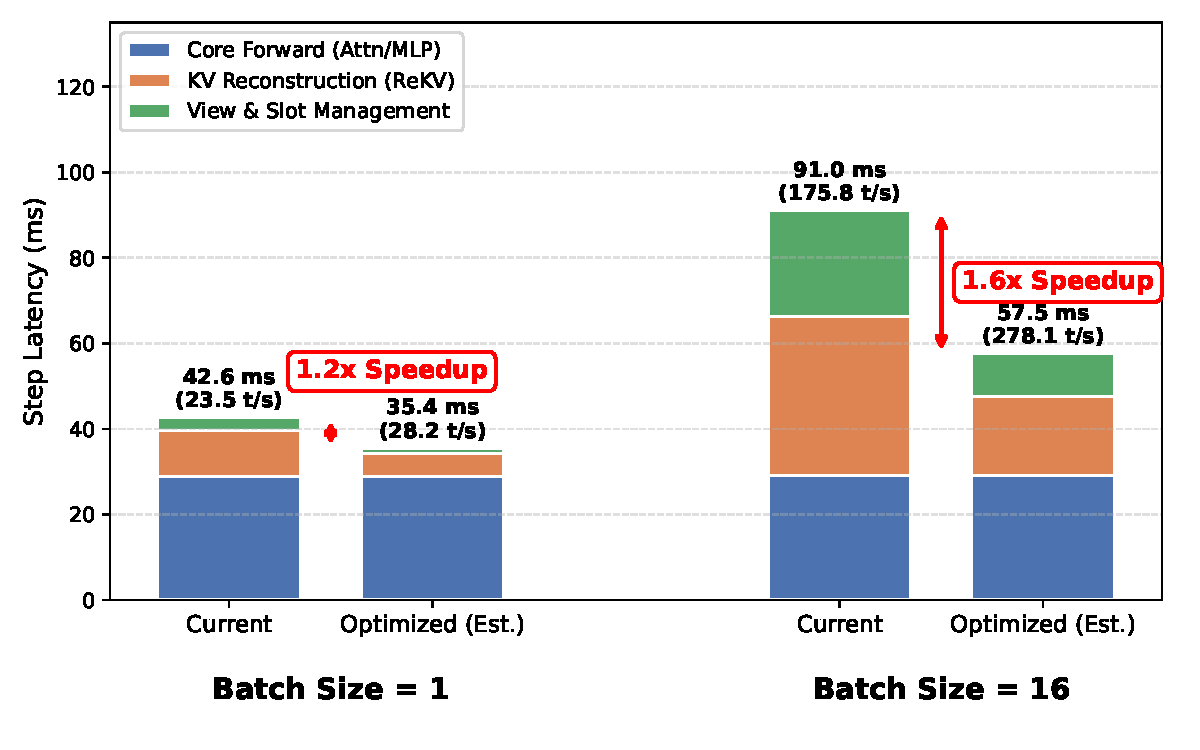
\includegraphics[width=0.7\textwidth]{figures/rekv_latency_comparison_bs1_vs_bs16.pdf} 
  % \vspace{-0.75em}
  \caption{Detailed latency breakdown and estimated speedup of Sparse-vLLM following kernel fusion, evaluated at a 128k context length with batch sizes of 1 and 16. \textbf{CUDA synchronization} was enabled at  points during testing for the purpose of latency analysis, which \textbf{incurs some performance overhead}.}
  \label{fig:latency_breakdown}
  % \vspace{-0.75em}
\end{figure*}

As illustrated in Figure~\ref{fig:latency_breakdown}, DeltaKV enables long-context inference under a tight memory budget, but the current prototype still incurs substantial \textit{runtime} overhead. At $BS=16$, the measured step latency is $91.0$\,ms, of which $37.3$\,ms is attributed to KV reconstruction and $24.7$\,ms to view/slot bookkeeping, leaving the remainder for model computation. To obtain stable and attributable timings, we insert CUDA synchronizations around key regions; this forces the host to wait for GPU completion and reduces overlap between kernel launches and other asynchronous work. As a result, the reported latencies should be interpreted as conservative (upper-bound) measurements of the current software stack, and can be higher than end-to-end throughput observed under fully asynchronous execution.

The bottleneck mainly stems from two factors: (1) \textit{Python-level control overhead}: sequence-wise logic, slot mapping, and dynamic view construction are executed serially in Python, triggering many small kernel launches and occasional host-device synchronization, with the impact growing with batch size. (2) \textit{Fragmented memory traffic}: reconstruction and bookkeeping are decomposed into multiple operators that materialize intermediate tensors in HBM; although some kernels are already fused, redundant global-memory reads/writes and launch overhead remain significant.

These costs indicate clear optimization opportunities via deeper operator fusion. A more integrated Triton/CUDA implementation could consolidate reconstruction (e.g., gather/de-RoPE, delta application, re-RoPE, and writeback) into fewer passes and move view/slot management onto GPU kernels, reducing both launch overhead and global-memory traffic by keeping temporaries in on-chip storage (registers/shared memory) when feasible. While the exact gain depends on hardware and workload, we expect that eliminating most Python-driven bookkeeping and further fusing reconstruction could reduce the $BS=16$ step latency to the $\sim55$--$60$\,ms range (about $1.5\times$--$1.7\times$ higher throughput), making the system more practical for large-scale long-context deployment.



% \subsection{Prefill Acceleration and Performance}
% \label{appendix:prefill_acc}

% DeltaKV is designed to be fully compatible with the prefill acceleration mechanism of OmniKV described in Appendix~\ref{app:sect:omnikv_method}.
% In our Sparse-vLLM implementation, we integrate the mean-aggregation selection policy directly into the \textit{Sparse Controller}.
% During the prefill phase of the filter layers, the controller computes the importance scores by averaging the attention weights along the query dimension.

% \paragraph{Impact on Accuracy}
% We evaluate the impact of this aggressive prefill pruning strategy on downstream tasks.
% As shown in Table~\ref{tab:longbench_prefill}, applying the prefill acceleration with DeltaKV results in negligible performance degradation on the LongBench benchmark compared to the full-cache baseline.
% This demonstrates that the mean-aggregation strategy effectively captures the essential information required for long-context understanding, while DeltaKV's residual compression ensures that the representation quality of these selected tokens remains high.

% % [PLACEHOLDER: Insert your LongBench Data Table here]
% % \begin{table}[h]
% %     \caption{LongBench Performance with Prefill Acceleration...}
% %     ...
% % \end{table}

% \paragraph{Prefill TTFT Analysis}
% By pruning the KV cache early in the prefill stage, DeltaKV avoids the overhead of storing and managing the full sequence history, leading to substantial improvements in processing speed.
% Table~\ref{tab:prefill_throughput} illustrates the prefill Time to First Token (TTFT) across different context lengths.
% Our method achieves a significant speedup compared to standard vLLM, particularly in ultra-long context scenarios where memory bandwidth is the primary bottleneck.

% % [PLACEHOLDER: Insert your Prefill Performance Table here]
% % \begin{table}[h]
% %     \caption{Prefill Throughput Comparison...}
% %     ...
% % \end{table}



\section{Brief Introduction to OmniKV}
\label{app:sect:omnikv_method}

OmniKV~\citep{hao2025omnikv} is a training-free framework designed to optimize KV cache memory usage and inference latency for long-context LLMs.
It operates on the core insight of \textit{Inter-Layer Attention Similarity}, which posits that the set of important tokens identified in a specific layer remains significant for subsequent layers.
Specifically, OmniKV designates a small subset of layers as ``filter layers'', denoted as $\mathbb{L}_{filter}$.
During the decoding phase, for any layer $l \in \mathbb{L}_{filter}$, the model computes the full attention scores using the current query and the entire historical KV cache.
Based on these scores, a Context Selector identifies the indices of the top-$k$ most relevant tokens, denoted as $\mathcal{I}_{topk}$.
For the subsequent layers that are not in $\mathbb{L}_{filter}$, OmniKV avoids full attention computation; instead, it selectively retrieves only the subset of keys and values corresponding to $\mathcal{I}_{topk}$ (i.e., $K_{\mathcal{I}_{topk}}$ and $V_{\mathcal{I}_{topk}}$) from the CPU-offloaded Context Bank to the GPU.
This dynamic context selection mechanism significantly reduces the GPU memory footprint and PCIe bandwidth overhead while maintaining model performance.

\paragraph{Prefill Acceleration via Chunking.}
Processing long prompts (e.g., >100k tokens) in a single forward pass often exceeds GPU memory limits.
To address this, OmniKV employs \textit{Chunk Prefill}, where the long input sequence is split into smaller segments (chunks) of length $L_q$ that are processed sequentially.
Consequently, during the prefill phase, the length of the queries ($L_q$) corresponds to the current chunk size, while the length of the Key/Value cache ($L_{kv}$) represents the accumulated history plus the current chunk, implying $L_q \le L_{kv}$.

To accelerate this phase without retaining the full history, OmniKV identifies important tokens by aggregating attention scores.
Formally, let $H$ denote the number of attention heads.
Given the attention score matrix $\mathbf{A} \in \mathbb{R}^{H \times L_q \times L_{kv}}$ computed in the filter layers for the current chunk, the importance score $s_{j}$ for the $j$-th KV token is derived by first averaging over the query length $L_q$ to capture temporal relevance, and then taking the maximum across the head dimension $H$ to retain the strongest signal:

\begin{equation}
    s_j = \max_{1 \le h \le H} \left( \frac{1}{L_q} \sum_{i=1}^{L_q} \mathbf{A}_{h, i, j} \right)
\end{equation}

By utilizing this score, OmniKV identifies the top-$k$ globally significant tokens from the current $L_{kv}$ candidates.
This strategy allows the model to discard less relevant tokens on-the-fly after processing each chunk, preventing memory explosion while preserving critical long-range context.


\section{Detailed Configurations}


\subsection{Benchmarks and Task Selection}
\label{app:sect:eval_details}

\paragraph{LongBench} Following the setting of AdaKV~\cite{feng2025adakv}, we utilize 16 datasets from LongBench covering Single/Multiple Document QA, Summarization, Few-Shot learning, Synthetic tasks, and Code generation. This benchmark primarily assesses single-turn dialogue capabilities.

\paragraph{SCBench} To evaluate the model's performance sustainability in realistic multi-turn dialogues, we employ SCBench. Due to computational resource constraints, we selected four representative tasks covering distinct categories: Retr.KV (String Retrieval), En.QA (Semantic Retrieval), ICL.ManyShot (Global Information), and Mix.Sum+NIAH (Multi-tasking).

\paragraph{AIME} We further verify the effectiveness of DeltaKV on complex reasoning tasks using the AIME benchmark, with a maximum output length set to 32,768 tokens.

\paragraph{Budget Ratio Setting} To ensure a fair comparison across methods, we enforce a budget ratio rather than a fixed token number. Consequently, the actual number of retained tokens is dynamically determined based on the prompt context length (Appendix~\ref{app:sect:kr_cr}).

\subsection{Efficiency Metrics}
\label{app:sect:kr_cr_def}
To quantify the trade-offs between memory saving and computational acceleration, we utilize two perspectives:
\begin{itemize}[nolistsep, left=0pt]
  \item \textbf{KV Cache Keep Ratio (KR):} Represents the percentage of KV cache stored in GPU memory relative to the full cache.
  
  \item \textbf{KV Cache Compute Ratio (CR):} Represents the percentage of tokens involved in the actual attention computation.
\end{itemize}
For specific calculation formulas regarding different baselines and DeltaKV, please refer to Appendix~\ref{app:sect:kr_cr}.

\subsection{Model Checkpoints}

We provide the specific Hugging Face model identifiers for all models evaluated in this work in Table~\ref{tab:model_ckpts}. The experiments were conducted using the official Instruct versions of Llama-3.1, the Qwen2.5 series (including the 1M context variant), and the DeepSeek-R1 distilled model.

\begin{table}[t]
\centering
\small
\caption{Model checkpoints used in our experiments.}
\label{tab:model_ckpts}
\begin{tabular}{lr}
\toprule
\rowcolor[HTML]{FFF2CC} \textbf{Model} & \textbf{Huggingface Model ID} \\
\midrule
Llama-3.1-8B-Instruct & \texttt{meta-llama/Llama-3.1-8B-Instruct}\\
Qwen2.5-7B-Instruct-1M & \texttt{Qwen/Qwen2.5-7B-Instruct-1M}\\
Qwen2.5-32B-Instruct & \texttt{Qwen/Qwen2.5-32B-Instruct}\\
DeepSeek-R1-Distill-Qwen-7B  & \texttt{deepseek-ai/DeepSeek-R1-Distill-Qwen-7B}\\
\bottomrule
\end{tabular}
\end{table}


\subsection{Detailed Setting of DeltaKV}
\label{subsec:detailed_settings}

\paragraph{Training Configuration.}
We train the DeltaKV modules using the AdamW optimizer with a learning rate of $2\text{e-}4$, a batch size of 1, and 1 gradient accumulation step. The learning rate schedule includes a linear warmup for the first 2\% of the training steps, followed by a linear decay to zero. 

\textit{Environment and Efficiency:} All experiments are implemented with \texttt{PyTorch} and \texttt{transformers}~\cite{wolf2020transformers} on a single NVIDIA RTX PRO 6000 (Blackwell). For Qwen2.5-32B-Instruct, we utilized \texttt{bitsandbytes} and gradient checkpointing~\cite{gradient_ckpt} to reduce memory consumption.
Training is efficient: for standard models (Llama-3.1-8B and Qwen2.5-7B), we trained on packed sequences of length 8,192 (160M tokens total) from \textbf{Fineweb-Edu}, completing in just \textbf{8 GPU hours}. The 32B model required 14 GPU hours. For the reasoning model (DeepSeek-R1-Distill), we sampled 8,000 sequences from \textbf{AM-DeepSeek-R1-Distilled-1.4M}, taking only 3.5 GPU hours.

\paragraph{Architecture and Hyperparameters.}
For the compression architecture, we set the compressed residual dimension $d_c$ to 25\% of the original KV dimension (i.e., $d_c = 0.25 \times 2d_k$). The compressor utilizes a hidden dimension of $d_h = 4096$ for the standard version. For the latency-optimized ``Light'' variant, we reduce the hidden dimension to $d_h = 3072$ and employ a SwiGLU-based encoder paired with a bias-free linear decoder. During retrieval, we select the top-$k=4$ nearest reference tokens from the history. The reference tokens are maintained with a stride of $s=10$, corresponding to a reference keep ratio of approximately 10\%.

\paragraph{Layer-wise Configuration.}
To maximize performance under strict memory budgets, we employ a hybrid strategy where a small subset of ``Full Attention Layers'' retain their complete KV cache, while the remaining layers are compressed using DeltaKV. The specific layer indices for full attention are manually selected based on importance profiling and are listed in Table \ref{tab:full_attn_layers_config}.

\begin{table}[t]
    \centering
    \caption{Configuration of Full Attention Layers for different models and budgets. Layers not listed are compressed.}
    \label{tab:full_attn_layers_config}
    % \resizebox{\columnwidth}{!}{%
    \begin{tabular}{ll}
        \toprule
        \rowcolor[HTML]{FFF2CC}
        \textbf{Model \& Setting} & \textbf{Full Attention Layer Indices} \\
        \midrule
        Llama-3.1-8B (30\% Budget) & 0, 1, 2, 8, 18 \\
        Llama-3.1-8B (20\% Budget) & 0, 1, 10, 18 \\
        Qwen2.5-7B (30\% Budget) & 0, 1, 2, 4, 7, 14 \\
        Qwen2.5-32B (20\% Budget) & 0, 1, 2, 3, 4, 5, 17, 29, 40 \\
        \bottomrule
    \end{tabular}%
    % }
\end{table}


\subsection{KR and CR Calculation}
\label{app:sect:kr_cr}

To comprehensively evaluate the efficiency of DeltaKV against existing approaches, we utilize two key metrics: KV Cache Keep Ratio (\textbf{KR}) and KV Cache Compute Ratio (\textbf{CR}). Let $r$ denote the target budget ratio (e.g., the percentage of tokens retained or selected for attention). The calculation methods for different categories of baselines and our proposed DeltaKV are formulated as follows:

\paragraph{Baselines}
Existing methods exhibit distinct trade-offs between memory footprint and computational overhead:
\begin{itemize}[nolistsep, left=0pt]
  \item \textbf{Static Eviction Methods (e.g., SnapKV, PyramidKV, AdaKV):} These methods permanently evict tokens to meet the budget constraint. Consequently, both the storage and the computation are reduced proportionally. Here, $r$ represents the sparsity ratio, indicating the proportion of the KV Cache that participates in each attention computation.
  \begin{equation}
    \text{KR} = r, \quad \text{CR} = r
  \end{equation}
    
  \item \textbf{Dynamic Selection Methods (e.g., OmniKV, Quest):} These approaches retain the full KV cache in GPU memory to preserve history but dynamically select only the top-$k$ important tokens for attention computation at each step.
  \begin{equation}
    \text{KR} = 100\%, \quad \text{CR} = r
  \end{equation}
    
  \item \textbf{Low-Rank Compression (e.g., Palu):} This method compresses the KV cache along the hidden dimension but typically requires reconstructing the full cache for attention computation, offering memory savings without computational acceleration.
  \begin{equation}
    \text{KR} = \frac{d_{\text{low}}}{d_{\text{orig}}}, \quad \text{CR} = 100\%
  \end{equation}
  where $d_{\text{low}}$ and $d_{\text{orig}}$ represent the compressed low-rank dimension and the original hidden dimension, respectively.
\end{itemize}

\paragraph{DeltaKV}
Our method employs a hybrid layer strategy, where $L_{\text{full}}$ layers perform standard full attention and $L_{\text{sparse}}$ layers utilize our residual compression with sparse attention.
\begin{itemize}[nolistsep, left=0pt]
  \item \textbf{KV Cache Keep Ratio (KR):} The memory footprint consists of the full cache for standard layers, and for sparse layers, the strided reference tokens (stride $s$) plus the compressed residuals (dimension $d_c$).
  \begin{equation}
    \text{KR}_{\text{DeltaKV}} = \frac{L_{\text{full}}}{L_{\text{sparse}}+L_{\text{full}}} + \frac{L_{\text{sparse}}}{L_{\text{sparse}}+L_{\text{full}}} \left( \frac{1}{s} + \frac{d_c}{2d_k} \right)
  \end{equation}
  where $L_{\text{sparse}}+L_{\text{full}}$ is the total number of layers and $2d_k$ is the dimension of the original KV Cache.

  \item \textbf{KV Cache Compute Ratio (CR):} DeltaKV adopts the same sparse attention mechanism as OmniKV for the compressed layers. Therefore, the computational cost is determined by the budget ratio $r$ applied in the sparse layers.
  \begin{equation}
    \text{CR}_{\text{DeltaKV}} = \frac{L_{\text{full}}}{L_{\text{sparse}}+L_{\text{full}}} \times 100\% + \frac{L_{\text{sparse}}}{L_{\text{sparse}}+L_{\text{full}}} \times r
  \end{equation}
\end{itemize}

\begin{table}[t]
    \centering
    \caption{KV Cache Keep Ratio (KR) and Compute Ratio (CR) Calculations for Llama-3.1-8B ($L=32$). Comparison between DeltaKV and Baselines under 30\% and 20\% Budgets.}
    \label{tab:deltakv_metrics_calc}
    \renewcommand{\arraystretch}{1.3} % Increase row height for better spacing
    \resizebox{\textwidth}{!}{%
    \begin{tabular}{llcccc}
        \toprule
        \rowcolor[HTML]{FFF2CC}
        \textbf{Budget} & \textbf{Method} & \textbf{Configuration Details} & \textbf{Formula Breakdown} & \textbf{KR (\%)} & \textbf{CR (\%)} \\
        \midrule
        
        % --- 30% Budget Section ---
        \multirow{6}{*}{\textbf{30\%}} 
        & SnapKV/PyramidKV & Static Eviction ($r=0.3$) & $\text{KR} = r$ & 30.0 & 30.0 \\
        & OmniKV/Quest & Dynamic Selection ($r=0.3$) & $\text{KR} = 100\%$ & 100.0 & 30.0 \\
        \cmidrule{2-6}
        & \multirow{4}{*}{\textbf{DeltaKV}} & $L_{\text{full}} = 5$ (Idx: 0, 1, 2, 8, 18) & \multirow{4}{*}{$\begin{aligned} 
            \text{KR} &= \tfrac{5}{32} + \tfrac{27}{32} \left( \underbrace{0.10}_{1/s} + \underbrace{0.25}_{d_c/2d_k} \right) \\ 
                      &= 0.156 + 0.844 \times 0.35 
        \end{aligned}$} & \multirow{4}{*}{\textbf{45.2}} & \multirow{4}{*}{\textbf{30.0}} \\
        & & $L_{\text{sparse}} = 27$ & & & \\
        & & $1/s = 0.10$ (Ref. Ratio) & & & \\
        & & $d_c/2d_k = 0.25$ (Comp. Rate) & & & \\
        
        \midrule
        
        % --- 20% Budget Section ---
        \multirow{6}{*}{\textbf{20\%}} 
        & SnapKV/PyramidKV & Static Eviction ($r=0.2$) & $\text{KR} = r$ & 20.0 & 20.0 \\
        & OmniKV/Quest & Dynamic Selection ($r=0.2$) & $\text{KR} = 100\%$ & 100.0 & 20.0 \\
        \cmidrule{2-6}
        & \multirow{4}{*}{\textbf{DeltaKV}} & $L_{\text{full}} = 4$ (Idx: 0, 1, 10, 18) & \multirow{4}{*}{$\begin{aligned} 
            \text{KR} &= \tfrac{4}{32} + \tfrac{28}{32} \left( \underbrace{0.10}_{1/s} + \underbrace{0.25}_{d_c/2d_k} \right) \\ 
                      &= 0.125 + 0.875 \times 0.35 
        \end{aligned}$} & \multirow{4}{*}{\textbf{43.1}} & \multirow{4}{*}{\textbf{20.0}} \\
        & & $L_{\text{sparse}} = 28$ & & & \\
        & & $1/s = 0.10$ (Ref. Ratio) & & & \\
        & & $d_c/2d_k = 0.25$ (Comp. Rate) & & & \\
        
        \bottomrule
    \end{tabular}%
    }
\end{table}

\paragraph{Settings}
Table \ref{tab:deltakv_metrics_calc} details the calculation of KV Cache Keep Ratio (KR) and Compute Ratio (CR) for Llama-3.1-8B ($L_{\text{sparse}}+L_{\text{full}}=32$) under 30\% and 20\% computation budgets. We compare DeltaKV against static eviction (e.g., SnapKV) and dynamic selection (e.g., OmniKV) baselines. For DeltaKV, we adopt a hybrid layer strategy where specific layers retain full attention based on importance profiling. In the 30\% budget setting, 5 layers (indices 0, 1, 2, 8, 18) are kept full ($L_{\text{full}}=5$), while the remaining 27 layers are compressed. In the 20\% budget setting, 4 layers (indices 0, 1, 8, 10) are kept full ($L_{\text{full}}=4$). The compressed layers utilize a residual compression rate of 25\% ($d_c/2d_k = 0.25$) and a reference token stride of $s=10$ ($1/s=0.10$). The analysis shows that DeltaKV achieves a significantly reduced memory footprint ($\text{KR} \approx 43\text{--}45\%$) compared to dynamic selection methods (100\% KR), while matching the efficient Compute Ratio (CR) of static baselines.


\section{Detailed and Other Experiments}

\subsection{LongBench}

In this section, we present the detailed experimental results on the LongBench benchmark. Tables~\ref{tab:longbench_detail_part1} and~\ref{tab:longbench_detail_part2} provide a comprehensive performance breakdown across all 16 datasets, covering Single-Document QA, Multi-Document QA, Summarization, Few-Shot Learning, Synthetic tasks, and Code generation. These results cover varying model scales, including Llama-3.1-8B-Instruct, Qwen2.5-7B-Instruct-1M, and Qwen2.5-32B-Instruct, offering a granular view of the aggregated metrics reported in the main text.

\begin{table*}[t]
\centering
\caption{Performance on Single-Doc QA, Multi-Doc QA, and Summarization tasks. Comparison with state-of-the-art baselines.}
\label{tab:longbench_detail_part1}
\resizebox{\textwidth}{!}{
\begin{tabular}{l cc cccc cccc cccc}
\toprule
\multirow{2.5}{*}{\textbf{Method}} & \multirow{2.5}{*}{\textbf{KR} $\downarrow$} & \multirow{2.5}{*}{\textbf{CR} $\downarrow$} & \multicolumn{4}{c}{\textbf{Single-Doc QA}} & \multicolumn{4}{c}{\textbf{Multi-Doc QA}} & \multicolumn{4}{c}{\textbf{Summarization}} \\
\cmidrule(lr){4-7} \cmidrule(lr){8-11} \cmidrule(lr){12-15}
 & & & \textbf{NQA} $\uparrow$ & \textbf{Qasp} $\uparrow$ & \textbf{MFQA} $\uparrow$ & \textbf{Avg.} $\uparrow$ & \textbf{HPQA} $\uparrow$ & \textbf{2WQA} $\uparrow$ & \textbf{Musq} $\uparrow$ & \textbf{Avg.} $\uparrow$ & \textbf{GovR} $\uparrow$ & \textbf{QMSm} $\uparrow$ & \textbf{MNew} $\uparrow$ & \textbf{Avg.} $\uparrow$ \\
\midrule
\multicolumn{15}{l}{\textbf{Llama-3.1-8B-Instruct}} \\
Full Cache & 100 & 100 & 32.2 & 46.6 & 56.9 & 45.3 & 58.1 & 48.0 & 32.4 & 46.2 & 34.3 & 24.9 & 27.0 & 28.7 \\
SnapKV & 30 & 30 & 31.0 & 45.3 & 57.2 & 44.5 & 57.4 & 49.0 & 32.9 & 46.4 & 30.0 & 25.1 & 24.3 & 26.5 \\
PyramidKV & 30 & 30 & 32.1 & 43.2 & 56.9 & 44.1 & 57.5 & 49.0 & 32.5 & 46.3 & 29.4 & 24.8 & 23.9 & 26.0 \\
Quest & 100 & 30 & 31.8 & 45.0 & 56.4 & 44.4 & 57.9 & 48.7 & 32.1 & 46.2 & 35.6 & 25.2 & 27.2 & 29.3 \\
KIVI & 25 & 100 & 31.1 & 46.5 & 56.7 & 44.8 & 58.0 & 49.2 & 31.4 & 46.2 & 34.3 & 25.5 & 27.2 & 29.0 \\
AdaKV & 30 & 30 & 31.6 & 45.2 & 57.1 & 44.7 & 58.7 & 48.3 & 32.5 & 46.5 & 30.6 & 24.7 & 24.3 & 26.6 \\
OmniKV & 100 & 30 & 31.6 & 46.0 & 56.8 & 44.8 & 58.1 & 48.2 & 32.1 & 46.1 & 34.3 & 25.2 & 27.0 & 28.9 \\
\quad +DeltaKV & 45 & 30 & 32.1 & 43.9 & 57.0 & 44.4 & 58.8 & 47.7 & 31.4 & 45.9 & 31.5 & 25.3 & 25.9 & 27.6 \\
\quad +DeltaKV$^\dagger$ & 45 & 30 & 29.5 & 44.3 & 55.8 & 43.2 & 57.4 & 49.7 & 33.3 & 46.8 & 32.4 & 25.4 & 25.5 & 27.7 \\
\quad\quad +4-bit & 29 & 30 & 30.5 & 43.2 & 56.2 & 43.3 & 57.6 & 49.3 & 33.0 & 46.6 & 31.6 & 25.0 & 25.3 & 27.3 \\
\midrule
\multicolumn{15}{l}{\textbf{Qwen2.5-32B-Instruct}} \\
Full Cache & 100 & 100 & 29.5 & 46.3 & 52.4 & 42.7 & 63.1 & 60.7 & 39.2 & 54.3 & 32.6 & 24.3 & 24.9 & 27.3 \\
SnapKV & 20 & 20 & 30.8 & 38.7 & 48.8 & 39.5 & 62.8 & 59.6 & 38.9 & 53.8 & 29.1 & 22.8 & 21.9 & 24.6 \\
OmniKV & 100 & 20 & 29.7 & 46.4 & 51.0 & 42.4 & 62.1 & 60.5 & 40.0 & 54.2 & 32.2 & 23.9 & 24.6 & 26.9 \\
\quad +DeltaKV & 44 & 20 & 30.0 & 44.3 & 51.4 & 41.9 & 62.3 & 61.2 & 39.2 & 54.2 & 30.4 & 23.7 & 24.4 & 26.2 \\
\midrule
\multicolumn{15}{l}{\textbf{Qwen2.5-7B-Instruct-1M}} \\
Full Cache & 100 & 100 & 29.4 & 47.7 & 50.3 & 42.5 & 60.4 & 54.8 & 33.4 & 49.6 & 35.5 & 24.4 & 25.9 & 28.6 \\
SnapKV & 30 & 30 & 28.8 & 46.1 & 50.3 & 41.7 & 59.3 & 53.5 & 33.5 & 48.8 & 32.8 & 24.0 & 23.0 & 26.6 \\
PyramidKV & 30 & 30 & 29.1 & 42.9 & 49.6 & 40.6 & 59.0 & 53.3 & 33.7 & 48.7 & 29.6 & 23.6 & 20.1 & 24.4 \\
Palu & 50 & 100 & 24.4 & 31.7 & 47.2 & 34.4 & 48.2 & 39.7 & 18.9 & 35.6 & 31.1 & 25.1 & 26.3 & 27.5 \\
OmniKV & 100 & 30 & 28.9 & 47.9 & 48.8 & 41.9 & 60.3 & 54.5 & 33.3 & 49.4 & 35.3 & 24.1 & 25.7 & 28.4 \\
\quad +DeltaKV & 48.9 & 30 & 29.2 & 46.7 & 49.6 & 41.8 & 59.5 & 53.5 & 33.9 & 49.0 & 33.8 & 24.2 & 25.0 & 27.7 \\
\bottomrule
\end{tabular}
}
\end{table*}


\begin{table*}[t]
\centering
\caption{Performance on Few-Shot, Synthetic, and Code tasks, with Overall Average. (Part 2 of Main Results).}
\label{tab:longbench_detail_part2}
\resizebox{\textwidth}{!}{
\begin{tabular}{l cc cccc ccc ccc c}
\toprule
\multirow{2.5}{*}{\textbf{Method}} & \multirow{2.5}{*}{\textbf{KR} $\downarrow$} & \multirow{2.5}{*}{\textbf{CR} $\downarrow$} & \multicolumn{4}{c}{\textbf{Few-Shot}} & \multicolumn{3}{c}{\textbf{Synthetic}} & \multicolumn{3}{c}{\textbf{Code}} & \multirow{2.5}{*}{\textbf{Avg.} $\uparrow$} \\
\cmidrule(lr){4-7} \cmidrule(lr){8-10} \cmidrule(lr){11-13}
 & & & \textbf{Trec} $\uparrow$ & \textbf{TQA} $\uparrow$ & \textbf{SamS} $\uparrow$ & \textbf{Avg.} $\uparrow$ & \textbf{Cnt} $\uparrow$ & \textbf{Retr} $\uparrow$ & \textbf{Avg.} $\uparrow$ & \textbf{LCC} $\uparrow$ & \textbf{Repo} $\uparrow$ & \textbf{Avg.} $\uparrow$ & \\
\midrule
\multicolumn{14}{l}{\textbf{Llama-3.1-8B-Instruct}} \\
Full Cache & 100 & 100 & 73.0 & 92.0 & 43.2 & 69.4 & 6.0 & 99.5 & 52.7 & 63.4 & 52.3 & 57.9 & 50.0 \\
SnapKV & 30 & 30 & 70.0 & 91.9 & 42.6 & 68.2 & 6.0 & 99.5 & 52.7 & 63.1 & 57.4 & 60.3 & 49.8 \\
PyramidKV & 30 & 30 & 71.0 & 91.7 & 42.9 & 68.5 & 5.7 & 99.5 & 52.6 & 62.3 & 56.0 & 59.1 & 49.5 \\
Quest & 100 & 30 & 73.0 & 90.5 & 43.6 & 69.0 & 6.6 & 99.5 & 53.1 & 59.9 & 55.3 & 57.6 & 50.0 \\
KIVI & 25 & 100 & 72.5 & 91.7 & 44.2 & 69.5 & 7.6 & 100.0 & 53.8 & 63.0 & 56.6 & 59.8 & 50.5 \\
AdaKV & 30 & 30 & 73.0 & 92.4 & 42.4 & 69.3 & 6.0 & 99.5 & 52.7 & 63.7 & 52.8 & 58.3 & 49.7 \\
OmniKV & 100 & 30 & 72.5 & 92.1 & 42.1 & 68.9 & 6.1 & 99.5 & 52.8 & 63.1 & 56.6 & 59.9 & 50.2 \\
\quad +DeltaKV & 45 & 30 & 73.0 & 92.3 & 43.6 & 69.7 & 6.8 & 100.0 & 53.4 & 63.5 & 57.0 & 60.2 & 50.2 \\
\quad +DeltaKV$^\dagger$ & 45 & 30 & 73.0 & 92.3 & 43.1 & 69.5 & 10.2 & 99.5 & 54.8 & 63.5 & 56.0 & 59.7 & 50.3 \\
\quad\quad +4-bit & 29 & 30 & 73.0 & 92.6 & 43.8 & 69.8 & 10.3 & 98.5 & 54.4 & 63.6 & 57.1 & 60.4 & 50.3 \\
\midrule
\multicolumn{14}{l}{\textbf{Qwen2.5-32B-Instruct}} \\
Full Cache & 100 & 100 & 72.0 & 84.5 & 46.5 & 67.6 & 12.0 & 100.0 & 56.0 & 50.9 & 34.3 & 42.6 & 48.4 \\
SnapKV & 20 & 20 & 71.0 & 84.1 & 46.4 & 67.2 & 12.0 & 100.0 & 56.0 & 49.2 & 34.1 & 41.7 & 47.1 \\
OmniKV & 100 & 20 & 71.5 & 83.7 & 46.4 & 67.2 & 12.3 & 100.0 & 56.1 & 49.2 & 34.2 & 41.7 & 48.1 \\
\quad +DeltaKV & 44 & 20 & 71.5 & 81.7 & 45.2 & 66.1 & 10.9 & 100.0 & 55.4 & 49.6 & 34.6 & 42.1 & 47.7 \\
\midrule
\multicolumn{14}{l}{\textbf{Qwen2.5-7B-Instruct-1M}} \\
Full Cache & 100 & 100 & 77.0 & 84.1 & 45.1 & 68.7 & 7.5 & 100.0 & 53.8 & 47.9 & 37.1 & 42.5 & 47.6 \\
SnapKV & 30 & 30 & 75.0 & 85.0 & 45.0 & 68.3 & 9.0 & 100.0 & 54.5 & 46.7 & 36.8 & 41.8 & 47.0 \\
PyramidKV & 30 & 30 & 74.5 & 84.2 & 44.5 & 67.7 & 9.0 & 100.0 & 54.5 & 44.7 & 36.5 & 40.6 & 46.1 \\
Palu & 50 & 100 & 76.0 & 86.4 & 43.7 & 68.7 & 2.5 & 87.5 & 45.0 & 20.2 & 22.4 & 21.3 & 38.8 \\
OmniKV & 100 & 30 & 77.5 & 85.4 & 44.3 & 69.1 & 8.0 & 100.0 & 54.0 & 46.1 & 36.8 & 41.5 & 47.4 \\
\quad +DeltaKV & 48.9 & 30 & 77.5 & 84.6 & 45.2 & 69.1 & 8.0 & 98.5 & 53.3 & 45.6 & 37.8 & 41.7 & 47.1 \\
\bottomrule
\end{tabular}
}
\end{table*}

\begin{table*}[t]
\centering
\caption{Component-wise ablation study on Llama-3.1-8B-Instruct (Part 1).}
\label{tab:ablation}
\resizebox{\textwidth}{!}{
\begin{tabular}{l cc cccc cccc cccc}
\toprule
\multirow{2.5}{*}{\textbf{Method}} & \multirow{2.5}{*}{\textbf{KR} $\downarrow$} & \multirow{2.5}{*}{\textbf{CR} $\downarrow$} & \multicolumn{4}{c}{\textbf{Single-Doc QA}} & \multicolumn{4}{c}{\textbf{Multi-Doc QA}} & \multicolumn{4}{c}{\textbf{Summarization}} \\
\cmidrule(lr){4-7} \cmidrule(lr){8-11} \cmidrule(lr){12-15}
 & & & \textbf{NQA} $\uparrow$ & \textbf{Qasp} $\uparrow$ & \textbf{MFQA} $\uparrow$ & \textbf{Avg.} $\uparrow$ & \textbf{HPQA} $\uparrow$ & \textbf{2WQA} $\uparrow$ & \textbf{Musq} $\uparrow$ & \textbf{Avg.} $\uparrow$ & \textbf{GovR} $\uparrow$ & \textbf{QMSm} $\uparrow$ & \textbf{MNew} $\uparrow$ & \textbf{Avg.} $\uparrow$ \\
\midrule
DeltaKV & 45 & 30 & 32.1 & 43.9 & 57.0 & 44.4 & 58.8 & 47.7 & 31.4 & 45.9 & 31.5 & 25.3 & 25.9 & 27.6 \\
\quad w/o $f_c$ and $f_d$  & 45 & 30 & 28.5 & 32.3 & 42.3 & 34.4 & 53.4 & 45.8 & 30.3 & 43.2 & 26.8 & 23.8 & 22.8 & 24.5 \\
\quad w/o Ref. Tokens $\mathcal{T}$ & 47 & 30 & 30.7 & 36.4 & 50.8 & 39.3 & 58.1 & 46.3 & 31.3 & 45.3 & 22.0 & 22.8 & 21.5 & 22.1 \\
\bottomrule
\end{tabular}
}
\end{table*}

\begin{table*}[t]
\centering
\caption{Component-wise ablation study on Llama-3.1-8B-Instruct (Part 2).}
\label{tab:ablation_part2}
\resizebox{\textwidth}{!}{
\begin{tabular}{l cc cccc ccc ccc c}
\toprule
\multirow{2.5}{*}{\textbf{Method}} & \multirow{2.5}{*}{\textbf{KR} $\downarrow$} & \multirow{2.5}{*}{\textbf{CR} $\downarrow$} & \multicolumn{4}{c}{\textbf{Few-Shot}} & \multicolumn{3}{c}{\textbf{Synthetic}} & \multicolumn{3}{c}{\textbf{Code}} & \multirow{2.5}{*}{\textbf{Avg.} $\uparrow$} \\
\cmidrule(lr){4-7} \cmidrule(lr){8-10} \cmidrule(lr){11-13}
 & & & \textbf{Trec} $\uparrow$ & \textbf{TQA} $\uparrow$ & \textbf{SamS} $\uparrow$ & \textbf{Avg.} $\uparrow$ & \textbf{Cnt} $\uparrow$ & \textbf{Retr} $\uparrow$ & \textbf{Avg.} $\uparrow$ & \textbf{LCC} $\uparrow$ & \textbf{Repo} $\uparrow$ & \textbf{Avg.} $\uparrow$ & \\
\midrule
DeltaKV & 45 & 30 & 73.0 & 92.3 & 43.6 & 69.7 & 6.8 & 100.0 & 53.4 & 63.5 & 57.0 & 60.2 & 50.2 \\
\quad w/o $f_c$ and $f_d$  & 45 & 30 & 66.0 & 90.0 & 41.7 & 65.9 & 10.1 & 100.0 & 55.1 & 60.6 & 53.9 & 57.2 & 46.7 \\
\quad w/o Ref. Tokens $\mathcal{T}$ & 47 & 30 & 55.5 & 90.8 & 40.5 & 62.3 & 7.0 & 94.5 & 50.8 & 59.0 & 51.8 & 55.4 & 45.9 \\
\bottomrule
\end{tabular}
}
\end{table*}

% \quad w/o Ref. Tokens $\mathcal{T}$
% \quad w/o $f_c$ and $f_d$


\subsection{SCBench}

We report the detailed subtask results for SCBench in Tables \ref{tab:scbench_detail_part1} and \ref{tab:scbench_detail_part2}. These tables illustrate the performance stability of DeltaKV across complex multi-turn scenarios, including Retrieval KV (R-1 to R-5), English QA (E-1 to E-7), Mixture of Summarization and NIAH (S-1 to S-10), and Many-Shot In-Context Learning (M-1 to M-5). The breakdown highlights the method's robustness in retaining critical information over long contexts compared to static eviction baselines.


\begin{table*}[t]
\centering
\caption{SCBench Results Part 1: Performance on Retrieval KV and English QA tasks. (R-x: Retrieval subtasks, E-x: English QA subtasks).}
\label{tab:scbench_detail_part1}
\resizebox{\textwidth}{!}{
\begin{tabular}{l cc c cccccc c ccccccc}
\toprule
\multirow{2.5}{*}{\textbf{Method}} & \multirow{2.5}{*}{\textbf{KR} $\downarrow$} & \multirow{2.5}{*}{\textbf{CR} $\downarrow$} & \multirow{2.5}{*}{\textbf{Avg.} $\uparrow$} & \multicolumn{6}{c}{\textbf{Retrieval KV}} & \multicolumn{8}{c}{\textbf{English QA}} \\
\cmidrule(lr){5-10} \cmidrule(lr){11-18}
 & & & & \textbf{Avg.} $\uparrow$ & \textbf{R-1} $\uparrow$ & \textbf{R-2} $\uparrow$ & \textbf{R-3} $\uparrow$ & \textbf{R-4} $\uparrow$ & \textbf{R-5} $\uparrow$ & \textbf{Avg.} $\uparrow$ & \textbf{E-1} $\uparrow$ & \textbf{E-2} $\uparrow$ & \textbf{E-3} $\uparrow$ & \textbf{E-4} $\uparrow$ & \textbf{E-5} $\uparrow$ & \textbf{E-6} $\uparrow$ & \textbf{E-7} $\uparrow$ \\
\midrule
\multicolumn{18}{l}{\textbf{Llama-3.1-8B-Instruct}} \\
Full Cache & 100 & 100 & 50.4 & 79.0 & 60.0 & 77.0 & 86.0 & 85.0 & 87.0 & 21.7 & 30.4 & 27.5 & 29.0 & 31.9 & 33.3 & 0.0 & 0.0 \\
SnapKV & 30 & 30 & 30.0 & 0.4 & 0.0 & 0.0 & 1.0 & 0.0 & 1.0 & 20.3 & 29.0 & 23.2 & 26.1 & 33.3 & 30.4 & 0.0 & 0.0 \\
OmniKV & 100 & 30 & 49.2 & 72.2 & 49.0 & 70.0 & 80.0 & 79.0 & 83.0 & 21.3 & 29.0 & 29.0 & 26.1 & 30.4 & 34.8 & 0.0 & 0.0 \\
\quad +DeltaKV & 45 & 30 & 45.0 & 58.0 & 38.0 & 51.0 & 68.0 & 62.0 & 71.0 & 20.5 & 27.5 & 29.0 & 21.7 & 31.8 & 33.3 & 0.0 & 0.0 \\
\quad +DeltaKV$^\dagger$ & 45 & 30 & 46.3 & 60.4 & 37.0 & 54.0 & 72.0 & 63.0 & 76.0 & 19.5 & 27.5 & 23.2 & 23.2 & 30.4 & 31.9 & 0.0 & 0.0 \\
\quad\quad+4-bit & 29 & 30 & 46.8 & 60.4 & 34.0 & 51.0 & 73.0 & 66.0 & 78.0 & 20.7 & 29.0 & 27.5 & 24.6 & 31.9 & 31.9 & 0.0 & 0.0 \\
\midrule
\multicolumn{18}{l}{\textbf{Qwen2.5-7B-Instruct-1M}} \\
Full Cache & 100 & 100 & 52.8 & 70.4 & 67.0 & 68.0 & 72.0 & 72.0 & 73.0 & 22.9 & 30.4 & 23.2 & 27.5 & 30.4 & 29.0 & 20.0 & 0.0 \\
SnapKV & 30 & 30 & 36.1 & 6.2 & 17.0 & 5.0 & 4.0 & 3.0 & 2.0 & 21.3 & 31.9 & 23.2 & 21.7 & 23.2 & 29.0 & 20.0 & 0.0 \\
OmniKV & 48 & 30 & 52.4 & 69.2 & 67.0 & 67.0 & 72.0 & 70.0 & 70.0 & 22.7 & 31.9 & 23.2 & 30.4 & 27.5 & 26.1 & 20.0 & 0.0 \\
\quad +DeltaKV & 48 & 30 & 50.6 & 59.4 & 54.0 & 60.0 & 63.0 & 59.0 & 61.0 & 24.0 & 36.2 & 27.5 & 27.5 & 30.4 & 26.1 & 20.0 & 0.0 \\
\quad +DeltaKV$^\dagger$ & 48 & 30 & 51.3 & 62.4 & 57.0 & 63.0 & 65.0 & 65.0 & 62.0 & 23.4 & 30.4 & 29.0 & 26.1 & 30.4 & 27.5 & 20.0 & 0.0 \\
\bottomrule
\end{tabular}
}
\end{table*}


\begin{table*}[t]
\centering
\caption{SCBench Results Part 2: Performance on Mixture of Summarization+NIAH and Many-Shot tasks. (S-x: Summ+NIAH subtasks, M-x: Many-Shot subtasks).}
\label{tab:scbench_detail_part2}
\resizebox{\textwidth}{!}{
\begin{tabular}{l cc c cccccccccc c ccccc}
\toprule
\multirow{2.5}{*}{\textbf{Method}} & \multirow{2.5}{*}{\textbf{KR} $\downarrow$} & \multirow{2.5}{*}{\textbf{CR} $\downarrow$} & \multicolumn{11}{c}{\textbf{Mix.Sum + NIAH}} & \multicolumn{6}{c}{\textbf{Many-Shot}} \\
\cmidrule(lr){4-14} \cmidrule(lr){15-20}
 & & & \textbf{Avg.} $\uparrow$ & \textbf{S-1} $\uparrow$ & \textbf{S-2} $\uparrow$ & \textbf{S-3} $\uparrow$ & \textbf{S-4} $\uparrow$ & \textbf{S-5} $\uparrow$ & \textbf{S-6} $\uparrow$ & \textbf{S-7} $\uparrow$ & \textbf{S-8} $\uparrow$ & \textbf{S-9} $\uparrow$ & \textbf{S-10} $\uparrow$ & \textbf{Avg.} $\uparrow$ & \textbf{M-1} $\uparrow$ & \textbf{M-2} $\uparrow$ & \textbf{M-3} $\uparrow$ & \textbf{M-4} $\uparrow$ & \textbf{M-5} $\uparrow$ \\
\midrule
\multicolumn{20}{l}{\textbf{Llama-3.1-8B-Instruct}} \\
Full Cache & 100 & 100 & 56.8 & 39.0 & 42.9 & 39.2 & 45.7 & 45.0 & 82.9 & 43.8 & 91.4 & 49.6 & 88.6 & 44.1 & 44.4 & 70.4 & 53.7 & 25.9 & 25.9 \\
SnapKV & 30 & 30 & 55.7 & 40.1 & 45.7 & 35.4 & 54.3 & 43.9 & 77.1 & 43.4 & 91.4 & 48.9 & 77.1 & 43.7 & 38.9 & 81.5 & 44.4 & 29.6 & 24.1 \\
OmniKV & 100 & 30 & 57.0 & 39.0 & 45.7 & 39.5 & 42.9 & 44.7 & 82.9 & 45.4 & 91.4 & 49.5 & 88.8 & 46.3 & 42.6 & 68.5 & 57.4 & 33.3 & 29.6 \\
\quad +DeltaKV & 45 & 30 & 50.0 & 37.3 & 28.6 & 35.7 & 8.6 & 42.9 & 74.3 & 44.2 & 91.4 & 48.0 & 88.6 & 51.5 & 46.3 & 74.1 & 59.3 & 35.2 & 42.6 \\
\quad +DeltaKV$^\dagger$ & 45 & 30 & 52.4 & 38.2 & 37.1 & 38.4 & 2.9 & 43.4 & 82.9 & 44.9 & 91.4 & 50.4 & 94.3 & 53.0 & 46.3 & 75.9 & 61.1 & 35.2 & 46.3 \\
\quad\quad +4-bit & 29 & 30 & 52.2 & 38.8 & 34.3 & 38.3 & 0.0 & 43.2 & 88.6 & 43.8 & 91.4 & 49.7 & 94.3 & 53.7 & 48.1 & 79.6 & 59.3 & 35.2 & 46.3 \\
\midrule
\multicolumn{20}{l}{\textbf{Qwen2.5-7B-Instruct-1M}} \\
Full Cache & 100 & 100 & 60.7 & 34.9 & 8.6 & 44.7 & 91.4 & 40.0 & 97.1 & 42.8 & 100.0 & 47.9 & 100.0 & 57.0 & 51.9 & 48.1 & 57.4 & 64.8 & 63.0 \\
SnapKV & 30 & 30 & 60.6 & 36.8 & 8.6 & 43.4 & 94.3 & 40.5 & 94.3 & 41.7 & 100.0 & 46.9 & 100.0 & 56.3 & 50.0 & 53.7 & 61.1 & 63.0 & 53.7 \\
OmniKV & 48 & 30 & 61.2 & 36.9 & 8.6 & 45.6 & 91.4 & 39.7 & 97.1 & 43.8 & 100.0 & 48.9 & 100.0 & 56.7 & 51.9 & 48.1 & 59.3 & 63.0 & 61.1 \\
\quad +DeltaKV & 48 & 30 & 60.6 & 35.2 & 8.6 & 41.4 & 94.3 & 40.7 & 100.0 & 41.8 & 100.0 & 47.3 & 97.1 & 58.5 & 53.7 & 48.1 & 59.3 & 63.0 & 68.5 \\
\quad +DeltaKV$^\dagger$ & 48 & 30 & 61.3 & 34.8 & 8.6 & 43.2 & 94.3 & 41.5 & 100.0 & 43.5 & 100.0 & 47.0 & 100.0 & 58.2 & 53.7 & 46.3 & 59.3 & 66.7 & 64.8  \\
\bottomrule
\end{tabular}
}
\end{table*}


